\chapter{Overview}
\thispagestyle{plain}
\label{Overview}

In this section we will briefly describe the android application, its publication mechanism, current threat landscape and algorithms that we would for classification.
\section{Android Applications}
\label{Android Applications}

Android applications are usually written in Java (although some have "native" C calls), and are distributed as APK (Android Package) files. Those APK files are in fact Zip archives, which contain compiled Java classes (in Dalvik DEX format), application resources, and an AndroidManifest.xml binary XML file containing application metadata. The APK also contains a public key and it’s associated $X.509$ certificate, bundled as a PKCS\#7 message in DER format.

\subsection{Naming conventions}
\label{Naming conventions}
When creating a new project, the Android developer documentation dictates that a full "Java-language-style" package name be used, and that developers "should use Internet domain ownership as the basis for package names (in reverse)~\cite{16}." This creates package names such as com.google.gmail for the mobile GMail application. To avoid name conflicts, package names must be unique across the entire universe of applications. Using reversed domain names theoretically limits potential namespace conflicts to a developer's own domain.

\subsection{Signing applications}
\label{Signing applications}
All Android applications must be cryptographically signed by the developer; an Android device will not install an application that is not signed. Typical Java tools, such as keytool and jarsigner, may be used to create a unique keypair and sign the mobile application.

In Android, the only key distribution mechanism used consists in bundling developer's public key with the application. Further, Android has no requirement for a keypair to be certified by a Certificate Authority (CA). In a study researchers~\cite{56} have observed that more than 99\% of the 76,480 applications they studied use self-signed certificates.

In other words, the primary purpose of the keypair is to distinguish between application authors, but not to provide any stronger security properties. In practice, keypairs are also used for:
\begin{itemize}
\item Ensuring that applications that are allowed to automatically update are signed by the same key as the previous version.
\item Potentially allowing applications signed by the same key to share resources.
\item Granting or denying permissions to a family of applications signed by the same key.
\item Removing all applications signed with the same key from the Android market and potentially from all connected devices when one of these applications is flagged as malware~\cite{57}.
\end{itemize}

On the other hand, due to the absence of any certification authority or PKI, signatures on Android do not provide any assurance about the identity of the signer. In essence, Android ensures that the AngeryBird application is correctly signed by somebody, but cannot prove that the Rovio Entertainment Ltd, the company behind the AngeryBird application, actually signed the AngeryBird application.

\section{Application Repackaging}
\label{Application Repackaging}
An existing application redistributed with a different signing key, often with functionality not present in the original version, is said to be repackaged. Some, all, or none, of the application's existing functionality can be preserved in the repackaged version.

\begin{figure}[h]
\centering
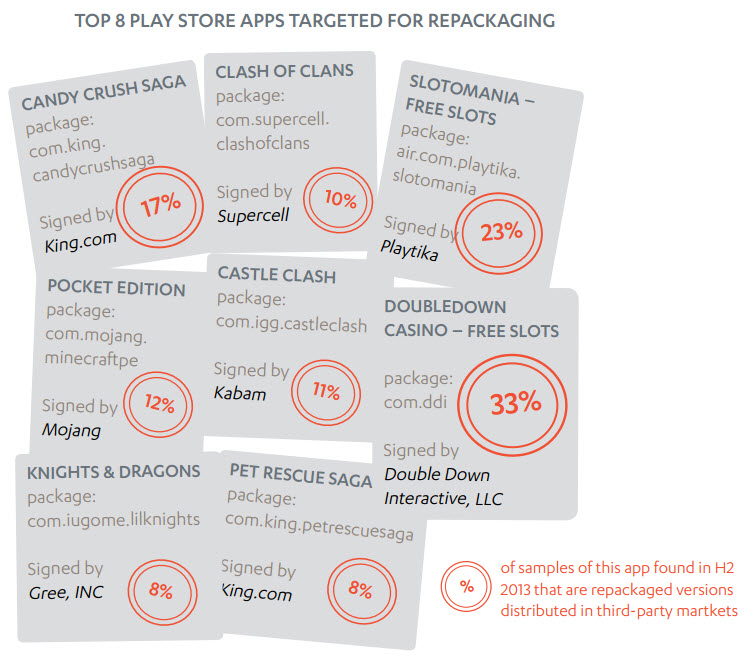
\includegraphics[width=\textwidth, height=0.6\textheight, keepaspectratio]{5_top_8_repacked.jpg}
\caption{Top 8 Repackaged Applications}
\label{fig:5_top_8_repacked}
\end{figure}

Applications can be repackaged for many reasons other than to distribute malware. For instance, a repackager may simply wish to
add advertising to an existing application to profit from somebody else's application. Application repackaging falls broadly in two
classes: spoofing and grafting. Figure \ref{fig:5_top_8_repacked} shows few of most popular repackaged applications found on android market places.

\subsection{Spoofing}
\label{Spoofing}
Mobile applications can simply be published under false pretenses, spoofing little or none of the features a legitimate application would possess. To deceive the user, a malicious program may advertise to be an existing application, or a non existent application that may plausibly exist, yet provide none of the expected functionality. As previously shown in peer-to-peer networks~\cite{58} and search-engine result poisoning~\cite{59,60}, this type of attack could flood a market with enough false positives to attract
users.

As an example, in July 2011, the legitimate Netflix application only supported specific devices and versions of Android. Unsupported devices could not locate and install the official application in the market. In October 2011, a fake version of the Netflix application was published in the official Android Market, claimed to "support" all devices, and thus appeared to owners of devices that could not download the legitimate application. The fake application displayed a plausible login screen, but then simply stole service credentials. Once credentials were entered, the application uninstalled itself~\cite{60}.

\subsection{Grafting}
\label{Grafting}
To achieve the desired functionality of a legitimate application, an attacker may elect to graft malware onto an existing
application, and subsequently republish the modified application. The attacker starts by downloading and extracting an existing
application. To do so, she unzips the APK archive to extract the application components (class files and manifest). Then, she adds malware to the application, and repackages it. Adding malware may require to reverse the DEX-formatted Java classes. While not entirely straightforward, tools such as undx~\cite{62}, baksmali, dedexer, or ded~\cite{63} can often successfully decompile .dex files to source code. DEX can also be converted to a typical Java jar collection of classes using the dex2jar utility,
at which point a typical Java decompiler can be used.

In the quite common case in which the .dex file does not need to be fully reversed to source code, much of the disassembly and
repackaging process can be automated. For instance, apktool~\cite{28} can unpack and repackage an existing .apk with two commands.
apktool has several side effects that result in non-required changes to the repackaged .apk. For instance, some files may be compressed in the repackaged application regardless of whether or not original file was compressed. With automatic compression the repackaged file may actually be smaller than the original despite the addition of malicious code. These side effects may be undesirable for an attacker that wishes for the application to remain as similar as possible to the original application.

In addition to the class files, the attacker may need to modify the AndroidManifest.xml, since this is where applicationlevel permissions are specified. This can be done using a tool such as AXMLPrinter2~\cite{64}. For instance, the malware to be added to the existing application may require the INTERNET or SEND\_SMS permissions, even if the permission is not specified in the original application.

Last, prior to publishing the "new" application to one or more markets, the attacker must cryptographically sign the application.
The signing can easily be performed with standard Java tools, e.g.,using jarsigner. Since Android uses self-signed certificates,
such signatures will pass installation-time checks.

\section{Current Android Malware Landscape}
\label{Current Android Malware Landscape}
Recent studies shows that Android system is increasingly being exploited by numerous malwares. Also most of these malwares are specifically created for android system. Figure ~\ref{fig:3_MobileThreatGraph2013} shows the recent mobile threat landscape. Also there is upward trend in using repackaged applications as a attack vector. Figure ~\ref{fig:4_malware-app-stores} shows that most of malicious apps come form third party market place. In 2013, Google play store found \~0.1\% applications to be malicious (136 from 132,798 unique applications recieved).

\begin{figure}
\centering
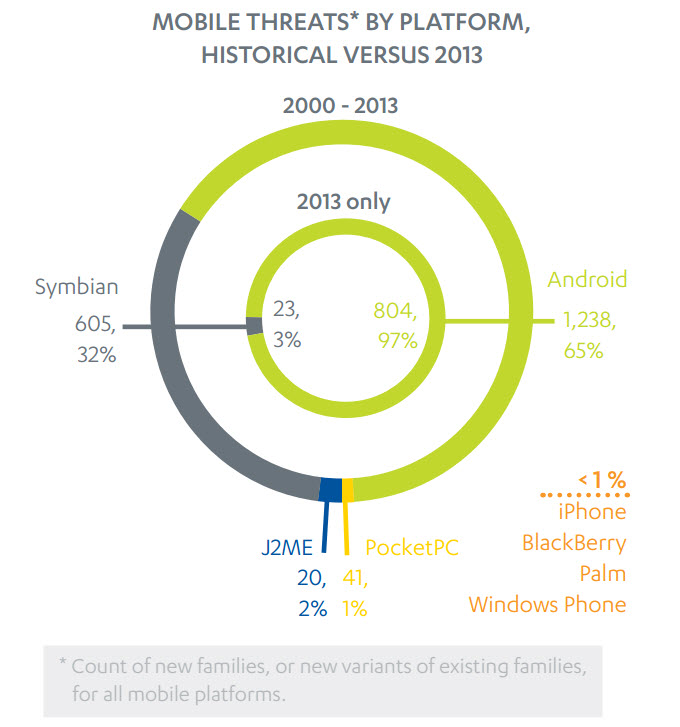
\includegraphics[width=\textwidth, height=0.5\textheight, keepaspectratio]{3_MobileThreatGraph2013}
\caption{Mobile Threats by Platform}
\label{fig:3_MobileThreatGraph2013}
\end{figure}
\begin{figure}
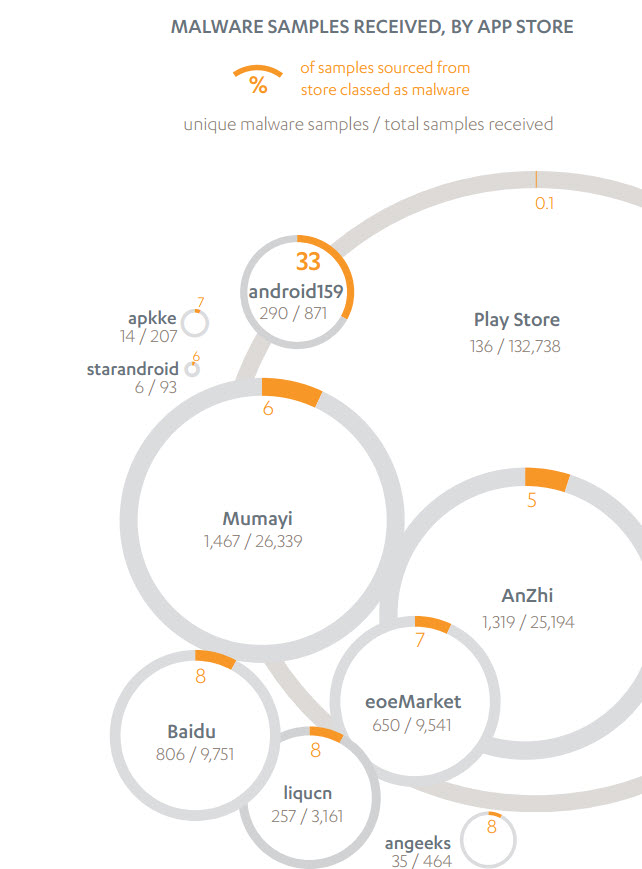
\includegraphics[width=\textwidth, height=\textheight, keepaspectratio]{4_malware-app-stores}
\caption{Android Malwares by Market Place}
\label{fig:4_malware-app-stores}
\end{figure}

\section{Boosting}
\label{Boosting}
`
Boosting is a machine learning technique for reducing the bias that
sometimes results from supervised learning~\cite{3}. The main idea is
to use an ensemble of weak learners to iteratively create a strong learner for
classification. Generally, boosting
algorithms consist of iteratively learning weak classifiers with
respect to a distribution and then combining them to construct a final
strong classifier with good classification performance. When the classifiers are
added, they are typically weighted in a way that is closely related
to the weak learners' accuracy. Every time a weak learner is added,
the fitted classification data used to recalculate the instance weights.
Input instances that are miss-classified gain weight,
and instances that are classified correctly lose weight. Thus, subsequent
weak learners focus more on the inputs that previous weak learners
miss--classified. We use AdaBoostM2 (which are discussed next) 
for classification of the malware specimens into families.

AdaBoost is the standard algorithm which is basis for AdaBoostM2.
AdaBoost, short for "Adaptive Boosting", is a machine
learning algorithm and can be used in conjunction with many other
learning algorithms to improve their performance. AdaBoost is adaptive
in the sense that subsequent classifiers built are corrected in favor
of those instances miss--classified by previous classifiers. AdaBoost is
sensitive to noisy data and outliers. In some problems, however, it
can be less susceptible to the over-fitting problem than most learning
algorithms. The classifiers that AdaBoost algorithm uses can be weak:
as long as their performance is slightly better than random, the
classification performance will improve the final model. AdaBoost
fits a new weak classifier in each of a series
of iterations $t=1,\ldots,T$. For each iteration $t$, a distribution of weights
$D_{t}$ is updated. The weights indicate the importance of each input instance
in the data set for the classification. For each iteration, the
weights of each incorrectly classified input are increased, and the
weights of each correctly classified input are decreased. This implies
that the new classifier focuses on the input which has so far been
miss--classified. The AdaBoost algorithm~\cite{4} which serves as the standard
base algorithm for other boosting techniques that we have used is
shown in the figure \ref{fig:ab1}.

\begin{figure}
\centering
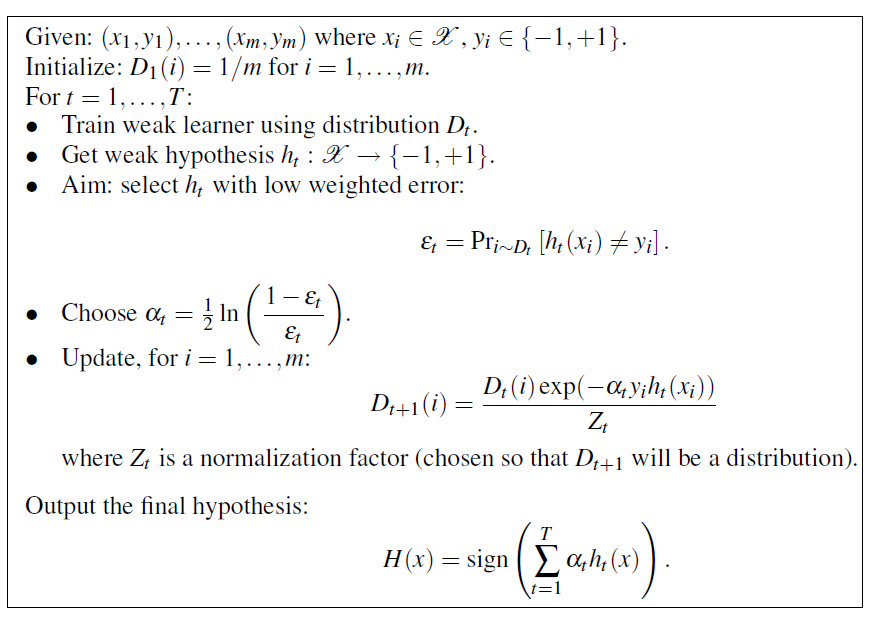
\includegraphics[width=14  cm] {ab1}
\caption{AdaBoost algorithm}
\label{fig:ab1}

\end{figure}

In the context of malware classification, for boosting, the frequencies of the syscalls in each document are taken as the features/predictors and the family names are taken as the responses/target classes. Similarly the word distribution in each file is calculated. In this case the frequencies of the words in each document are taken as the features and the corresponding family names are taken as responses. The performance of the classification using the boosting algorithm AdaBoostM2 are compared with other algorithms. We experimentally evaluate the classification performance of AdaBoostM2 for malware family prediction.


\subsection{AdaBoostM2}
\label{AdaBoostM2}
AdaBoostM2 is an extension of the standard AdaBoost algorithm. This
boosting algorithm is designed for multi--class problems with weak base
classifiers. The algorithm is designed to minimize a loose bound on
the training error. Since there are multiple classes of metamorphic
malware, we opt for AdaBoostM2. In AdaBoostM2, first, we allow the
weak learner to generate more expressive hypotheses, which, rather
than identifying a single class label, instead choose a set of
plausible labels. This may often be easier than choosing just one
class label. It is seen that the boosting algorithm AdaBoostM2, achieves
boosting if each weak hypothesis has pseudo-loss slightly better than
random guessing.

Rather than using the usual prediction error, we settle for having the weak
hypotheses do well with respect to a more sophisticated error measure
that we call the pseudo-loss. Unlike ordinary error which is computed
with respect to a distribution over examples, pseudo-loss is computed
with respect to a distribution over the set of all pairs of examples
and incorrect labels. In the algorithm~\cite{4} described in figure
\ref{fig:ab}, B is a set of all mislabels. On each round
$t$ of boosting, AdaBoostM2 supplies the weak learner
with a mislabel distribution $D_t$. In response, the weak
learner computes the hypothesis $h_t$. Intuitively, we
interpret each mislabel $(i,y)$ as representing the binary question of
the form: Do you predict the label associated with $x_i$
is $y_i$ (correct) or $y$ (incorrect)? The weak learner’s
goal is to find the weak hypothesis $h_t$ with small
pseudo loss. Then the distribution $D_t$ is updated with
this pseudo-loss. After $T$ iterations, the final hypothesis for
AdaBoostM2 is formulated.

\begin{figure}
\centering
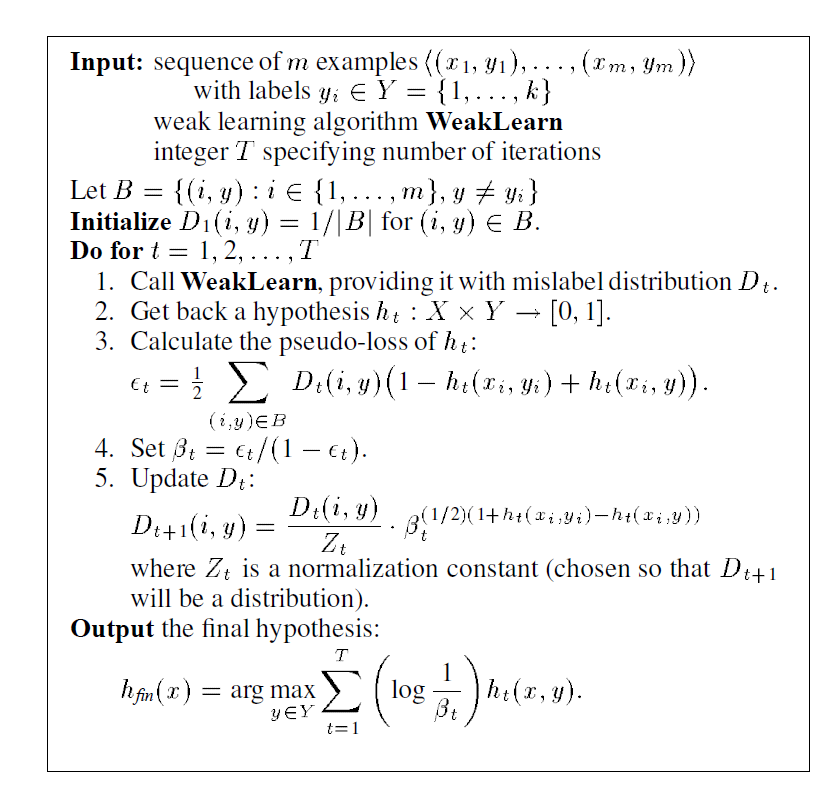
\includegraphics[width=\textwidth, height=\textheight, keepaspectratio] {ab}
\caption{AdaBoostM2 algorithm}
\label{fig:ab}
\end{figure}


\section{Stacked Denoising Autoencoder (SdA)}
\label{Stacked Denoising Autoencoder}

\subsection{Notations}
\label{Notations}
Let \(X\) and \(Y\) be two random variables with joint probability density \( p(X,Y)\), with marginal distributions \(p(X)\) and \(p(Y)\). Throughout the text, we will use the following notation:
	\begin{description}
	\item Expectation: \(E_{p(X)}[f(x)]=\int{p(x)\,f(X)\,dx}\) where \(y=f(x)=s(Wx + b)\) 
	\item Entropy: \(H(X)=H(p)=E_{p(X)}[\ -log\ p(X)\ ]\)
	\item Conditional entropy: \(H(X|Y) = E_{p(X,Y)} [\ -log\ p(X|Y)\ ]\)
	\item Kullback-Leibler divergence: \(DKL(pkq) = E_{p(X)}[\ log\ p(X)q(X)\ ] \)
	\item Cross-entropy: \(H(pkq) = Ep(X)[-\ log\ q(X)] = H(p)\ + DKL(pkq) \)
	\item Mutual information: \( (X;Y) = H(X) - H(X|Y ) \)
	\item Sigmoid: \( s(x) = \frac{1}{1+e^{-x}} \)\ and \(s(x) = (s(x1), \ldots, s(xd))^{T} \)
	\item Bernoulli distribution with mean \(u:B_{u}(x)\)\ and by extension \(B_{u}(x)=(B_{u1}(x1),\ldots, B_{ud}(xd)) \)
	\end{description}
The setup we consider is the typical supervised learning setup with a training set of \(n(input, target)\) pairs \(Dn = {(x(1), t(1)),\ldots, (x(n), t(n))}\), that we suppose to be an i.i.d. sample from an unknown distribution \(q(X, T)\) \ with corresponding marginals \(q(X)\) and \(q(T)\).

\subsection{The Basic Autoencoder}
\label{The Basic Autoencoder}

We begin by recalling the traditional autoencoder model such as the one used in~\cite{30} to build deep networks. An autoencoder 
takes an input vector \(x \in [0, 1]^d\), and first maps it to a hidden representation \(y \in [0, 1]^{d'}\) through a 
deterministic mapping \(y = f(x) = s(Wx + b)\), parametrized by \(\theta = {W, b}\). $W$ is a \(d' \times d\) weight matrix and $b$ 
is a bias vector. The resulting latent representation $y$ is then mapped back to a "reconstructed" vector \(z = g_{\theta'}(y) = s(W'_{y} + b') \) with \(\theta' = {W', b'}\). The weightmatrix $W'$ of the reverse mapping may optionally be constrained by \(W' = W^T\) ,in which case the autoencoder is said to have tied weights. Each training \(x^i\) is thus mapped to a corresponding \(y^i\) and a reconstruction \(z^i\). The parameters of this model are optimized to minimize the average reconstruction error:
\begin{equation}\label{eq:sdearmin}
\centering
\begin{aligned}
{\theta}^*, {\theta'}^* &= {\Large\substack{arg\, min \\ {\theta, \theta'}}}\frac{1}{n} \sum_{i=1}^{n} L(x^{(1)}, z^{(i)})\\
&= {\Large\substack{arg\, min \\ {\theta, \theta'}}}\frac{1}{n} \sum_{i=1}^{n} L\left(x^{(i)}, g_{\theta'}(f_{\theta}(x^{(i)}))\right) 
\end{aligned}
\end{equation}

where $L$ is a loss function such as the traditional squared error \(L(x,z) = {||x-z||}^2\). An alternative loss, suggested by the interpretation of $x$ and $z$ as either bit vectors or vectors of bit probabilities (Bernoullis) is the \(reconstruction cross entropy\):
\begin{equation}\label{eq:sdeburarmin}
\centering
\begin{aligned}
L_{H}(X,Z) &= H(B_X||B_Z) \\
&= -\sum_{k=1}^d\left[X_k\ logZ_k+(1-X_k)\ log\left(1-Z_k\right)\right]
\end{aligned}
\end{equation}

\begin{figure}
\centering
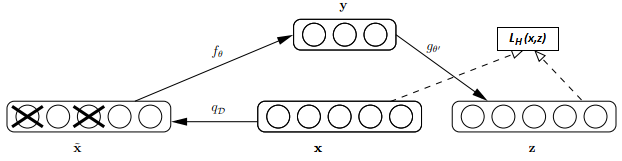
\includegraphics {sda_algo.png}
\caption{An example x is corrupted to \(\widetilde{x}\). The autoencoder then maps it to y and attempts to reconstruct x.}
\label{fig:sda_algo}
\end{figure}

Note that if x is a binary vector, $L_H(x, z)$ is a negative log-likelihood for the example $x$, given the Bernoulli parameters $z$. Equation ~\ref{eq:sdearmin} with $L = L_H$ can be written 
\begin{equation}\label{eq:sdearmin}
\centering
\begin{aligned}
{\theta}^*, {\theta'}^* &= {\Large\substack{arg\, min \\ {\theta, \theta'}}} E_{q^0(X)}\ \left[L_H\left(X, g_{\theta'}(f_{\theta}(X))\right)\right]
\end{aligned}
\end{equation}
where \(q^0(X)\) denotes the empirical distribution associated to our $n$ training inputs. This optimization will typically be carried out by stochastic gradient descent.
\subsection{The Denoising Autoencoder}
\label{The Denoising Autoencoder}
To test our hypothesis and enforce robustness to partially destroyed inputs we modify the basic autoencoder we just described. We will now train it to reconstruct a clean “repaired” input from a corrupted, partially destroyed one. This is done by first corrupting the initial input $x$ to get a partially destroyed version \(\widetilde{x}\) by means of a stochastic mapping \(\widetilde{x} \tilde q_D(\widetilde{x}|x)\).

In our experiments, we considered the following corrupting process, parametrized by the desired proportion $v$ of “destruction”: for each input $x$, a fixed number $vd$ of components are chosen at random, and there value is forced to 0, while the others are left
untouched. The procedure can be viewed as replacing a component considered missing by a default value, which is a common technique. A motivation for zeroing the destroyed components is that it simulates the removal of these components from the input. For our examples, this corresponds to “salt noise”. Note that alternative corrupting noises could be considered. The corrupted input ˜\(\widetilde{x}\) is then mapped, as with the basic autoencoder, to a hidden representation \(y = f_{\theta}(\widetilde{x}) = s(W\widetilde{x} + b)\) from which we reconstruct a \(z = g_{\theta'}(y) = s({W'}_y + b') \) (refer ~\ref{fig:sda_algo} schematic process). As before the parameters are trained to minimize the average reconstruction error \(L_{H}(X,Z) = H(B_X||B_Z)\) over a training set, i.e. to have $z$ as close as possible to the uncorrupted input $x$. But the key difference is that $z$ is now a deterministic function of ˜\(\widetilde{x}\) rather than x and thus the result of a stochastic mapping of x. 

Let us define the joint distribution: 
\( q^0(X,\widetilde{X},Y) = q^0(X)q_D(\widetilde{X}|X)\delta_{f_{\theta}(\widetilde{X})}(Y) \)
where \(\delta_u(v)\) puts mass 0 when \(u \ne v\). Thus $Y$ is a deterministic function of \(\widetilde{X}\). The \(q^0(X,\widetilde{X},Y)\) is parametrized by $\theta$. The objective function minimized by stochastic gradient descent becomes:
\begin{equation}\label{eq:sdearmin}
\centering
\begin{aligned}
{\theta}^*, {\theta'}^* &= {\Large\substack{arg\, min \\ {\theta, \theta'}}} E_{q^0(X,\widetilde{X})}\ \left[ L_H\left(X, g_{\theta'}(f_{\theta}(\widetilde{X}))\right)\right]
\end{aligned}
\end{equation}
So from the point of view of the stochastic gradient descent algorithm, in addition to picking an input sample from the training set, we will also produce a random corrupted version of it, and take a gradient step towards reconstructing the uncorrupted version from the corrupted version. Note that in this way, the autoencoder cannot learn the identity, unlike the basic autoencoder, thus removing the constraint that \(d' < d \) or the need to regularize specifically to avoid such a trivial solution.
%\begin{flushleft}

